\documentclass[a4paper]{article}

\usepackage[english, serbian]{babel}
\usepackage[utf8]{inputenc}
\usepackage{authblk}
\usepackage{graphicx}
\usepackage{xcolor}
\usepackage{amsmath}
\usepackage{amssymb}
\usepackage{amsfonts}
\usepackage{enumitem}
\usepackage{multicol}
\usepackage{hyperref}

\usepackage[backend=bibtex, style=numeric]{biblatex}
\addbibresource{references.bib}

\graphicspath{ {images/} }

\title{Automatsko prevođenje}
\author{Vladimir Vuksanović}
\affil{Matematički fakultet}
\date{}

\begin{document}

\maketitle

% Uvodni deo koji sadrži opis problema koji se rešava sa pregledom literature i naučne doprinose drugih istraživača na polju rešavanja razmatranog problema.
\section{Uvod}

Automatsko prevođenje podrazumeva prevođenje teksta sa jednog prirodnog jezika na drugi korišćenjem kompjutera. Preciznije, potrebno je za ulaznu recenicu proizvoljne duzine na izvornom jeziku generisati izlaznu recenicu, ne nuzno iste duzine, na ciljnom jeziku koja ima isto znacenje kao ulazna. 

Za resavanje ovog problema cemo koristiti NMT (neural machine translation) pristup koji koristi neuronsku mrezu da predvidi sekvencu reci u prevodu. 
Kako su ulaz i izlaz sekvence koje mogu biti proizvoljnih duzina, prevodjenje pripada grupi sequence-to-sequence problema. To onemogucava koriscenje potpuno povezane mreze koja zahteva fiksan broj ulaza i izlaza. 
Standardni pristup za rešavanje ovog problema je korišćenjem enkoder-dekoder arhitekture opisane u \cite{sutskever2014sequence} i \cite{cho2014learning} koja u kombinaciji sa rekurentnom neuronskom mrezom daje dodatnu fleksibinost koja je prethodno nedostajala. Ova arhitektura u praksi daje veoma dobre rezultate i koristi je jedan od najpoznatijih servisa ovog tipa, \href{https://translate.google.com/}{Google Translate} \cite{wu2016googles}. 
Osnovna ideja je da enkoder od ulazne sekvence generise reprezentaciju \textit{fiksne} duzine prolaskom rec po rec kroz LSTM sloj. Ta reprezentacija se kasnije koristi u dekoderu kao polazna tacka za generisanje prevoda na ciljni jezik analognim postupkom. Dodatno, primeceno je da se obrtanjem redosleda reci u ulaznoj recenici bolje ocuvaju veze izmedju reci, sto ce biti primenjeno u implementaciji.

% Opis vašeg rešenja zadatog problema. Ovim poglavljem opišite sve relevantne aspekte vašeg rada: npr. opšti rad algoritma, način kodiranja rešenja i funkciju cilja u slučaju da radite optimizacionu tehniku, itd. Budite objektivni i pošteni u opisu svoje metode i jasno ukažite na to da ste reprodukovali pristup koji je neko već osmislio pre vas tako što ćete ubaciti odgovarajuće reference ka svim relevantnim radovima (ovo je potpuno normalna situacija i ne podrazumeva nikakvo smanjivanje poena).
\section{Implementacija}

%referisati na papir i keras.io primer
Model je implementiran u programskom jeziku Python uz koriscenje keras biblioteke. Implementacija prati osnovne korake sa zvanicnog sequence-to-sequence primera sa keras veb stranice \cite{} pri cemu se predikcija vrsi na nivou reci umesto pojedinacnih slova.

\subsection{Pretprocesiranje}
Podaci za trening se sastoje od recenica na izvornom jeziku i njihovih prevoda na ciljni jezik. Posto direktna upotreba recenica u tekstualnom obliku nije pogodna, moracemo da ih pretvorimo u reprezentaciju koja bolje radi sa neuronskom mrezama.

Prvi korak pretprocesiranja je eliminisanje specijalnih simbola iz recenica jer nam oni nisu korisni prilikom prevodjenja.
Dalji koraci se primenjuju odvojeno za ulazne i izlazne recenice.
Kako bi recenice mogle da se upotrebe kao ulaz neuronske mreze potrebno je predstaviti ih kao niz brojeva. To se radi jednostavnim pridruzivanjem broja svakoj reci iz trening skupa ili nekog predefinisanog recnika u kom slucaju se dodaje i token za nepoznate (out-of-vocabulary) reci. Ovaj proces se naziva tokenzacija.
Za ulazne recenice uvodimo dodatni korak obrtanja redosleda tokena u sekvenci zato sto se tako bolje ocuvaju veze iizmedju reci u duzim recenicama.
Sve recenice iz respektivnih skupova se potom dopunjavaju "praznim" tokenima dok ne postanu iste duzine. Ulazne recenice se dopunjuju sa leve strane, a izlazne sa desne.
Na kraju, potrebno je napraviti dva tipa izlaznih recenica, jedan tip predstavlja ulaz u dekoder a drugi predstavlja izlaz. Prva rec koju dekoder treba da dobije je pocetni (start of sequence) token i on se dodaje na pocetak svake recenice koja ulazi u dekoder. Analogno, na recenice koje predstavljaju izlaz iz dekodera potrebno je dodati zavrsni (end of sequence) token. Ostatak postupka je isti kao za ulazne recenice.

\subsection{Enkoder}
Enkoder je zaduzen da na osnovu dobijene sekvence generise reprezentaciju fiksne duzine koja bi trebalo da sadzi sve informacije potrebne da se konstruise prevod na ciljnom jeziku. Ulaz u enkoder je tensor dimenzije $n \times m$ gde je $n$ broj recenica, a $m$ duzina ulazne sekvence. Ulaz je vezan za embedding sloj koji svakoj reci dodeljuje vektor fiksne duzine tako da udaljenost izmedju vektora zavisi od znacenja reci. Umensto da model uci reprezentacije za vreme treninga, koristimo GloVe \cite{} model treniran na 5 biliona reci sa vikipedije gde je vektor duzine 100. Na kraju se pomocu LSTM sloja dobija konacni vektor dimenzije 256.

\subsection{Dekoder}
Dekoder koristi svoje unutrasnje stanje i prethodno generisanu rec kako bi odredio sledecu rec u recenici. Po strukturi dekoder je veoma slican enkoderu. Ulazni sloj sada ima drugu dimenziju jednaku duzini izlazne sekvence dok embedding i LSTM slojevi ostaju nepromenjeni. Na kraju se nadovezuje na potpuno povezani sloj sa softmax aktivacijom koji odredjuje verovatnocu za svaku rec na ciljnom jeziku.

Inicijalno se kao unutrasnje stanje koristi izlaz iz enkodera, a kao prethodno generisanu rec uzimamo pocetni (\textless sos\textgreater) token koji je uveden prilikom pretprocesiranja. Dekodiranje se prekida ili dok se ne dobije zavrsni (\textless eos\textgreater) token ili dok se ne dostigne zadata maksimalna duzina recenice.

\subsection{Model}

Kombinovanjem prethodno opisanog enkodera i dekodera tako da dekoder inicijalno dobije stanja iz enkodera, dobija se konacni model.

\begin{figure}[h!]
  \centering
    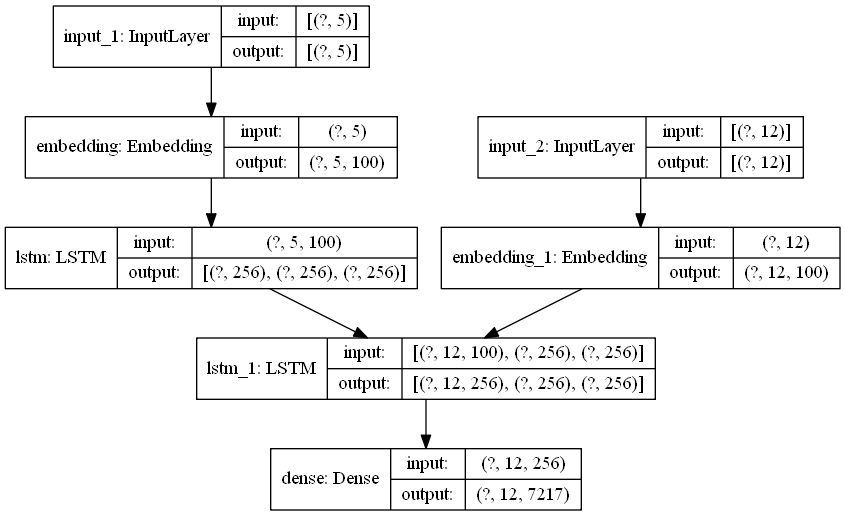
\includegraphics[width=\textwidth]{model}
  \caption{Konacan izgled modela}
  \label{fig:model}
\end{figure}

Optimizator koji koristimo je \textit{rmsprop}, funkcija gubitka je kategorijska unakrsna entropija, a metrika koju pratimo je tacnost.

\subsection{Trening}

Opisani model je treniran na 20.000 parova recenica na engleskom i francuskom jeziku iz skupa preuzetog sa \cite{manythings} koji je deo \href{https://tatoeba.org/eng}{Tatoeba projekta}. Model je treniran na 10 epoha sa velicinom grupe od 128 instanci i 10\% skupa za validaciju. Posto ceo skup obradjenih podataka ne moze da stane u radnu memoriju za vece skupove odjednom, koristimo generator da konstruisemo batch po batch.

Za treniranje je koricena Google Colaboratory platforma i trajalo je 3 sata.

\subsection{Generisanje prevoda}

Prethodni model radi samo ako vec na samom pocetku imamo celu prevedenu recenicu sto je dobro za vreme treniranja modela ali je neupotrebljivo za potrebe prevodjenja novih recenica. Iz tog razloga pravimo novi model koji koristi vec trenirane delove iz prethodnog modela ali sa modifikovanim dekoderom. Ulaz u novi dekoder je samo jedna rec koja se inicijalno postavlja da bude pocetni token. Sada je moguce iterativno pozivati dekoder sve dok se ne dodje do zavrsnog tokena ili nekog odredjenog limita na duzinu recenice.

\begin{figure}[h!]
  \centering
    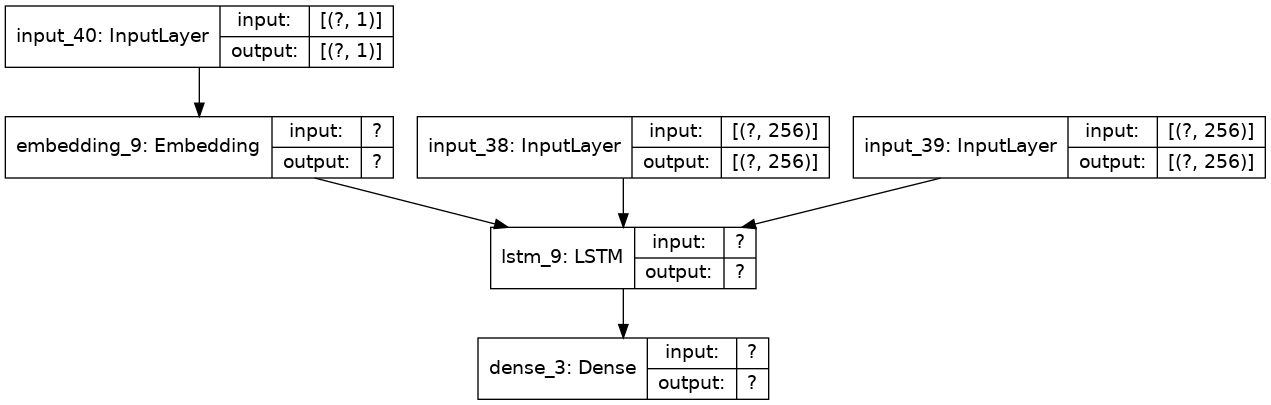
\includegraphics[width=\textwidth]{inference_model}
  \caption{Model za prevodjenje}
  \label{fig:inference_model}
\end{figure}

Umesto da se prevod trazi gramzivo, rec po rec, koristicemo algoritam \textit{beam search} pretrage.
Prvo se bira parametar $B$ koji predstavlja broj reci koje zelimo da budu razmatrane kao prva rec. Kada se izabere prvih $B$ kandidata, za svaku od njih se potom predvidja druga rec trazeci par koji je najverovatniji. Ovaj postupak se ponavlja do kraja prevoda. Specijalno, za vrednost $B = 1$ postupak se svodi na gramzivu pretragu. Formalno, algoritam maksimizira vrednost funkcije
$$argmax\prod_{t=1}^{Ty} P(y^{<t>}|X, y^{<1>}, y^{<2>}, ..., y^{<t-1>})}$$
Kako su sve verovatnoce izmedju 0 i 1, prethodni proizvod brzo postaje veoma mali broj. Zbog toga se umesto obicnog proizvoda koristi proizvod logaritama.
$$argmax\prod_{t=1}^{Ty} \log P(y^{<t>}|X, y^{<1>}, y^{<2>}, ..., y^{<t-1>})}$$
Jos jedan problem sa ovim formulama je sto favorizuju krace recenice zato sto se svakim mnozenjem smanjuje verovatnoca prevoda. Da bi kompenzovali za ovo normalizovacemo formulu tako sto je podelimo sa brojem reci u prevodu. Ovo je konacna formula koju koristimo.
$$argmax \frac{1}{Ty} \prod_{t=1}^{Ty} \log P(y^{<t>}|X, y^{<1>}, y^{<2>}, ..., y^{<t-1>})}$$

Od izbora parametra $B$ zavisi koliko potencijalnih prevoda ce biti razmatrano i time celokupni kvalitet prevoda. Sto je parametar veci, vise izbora se razmatra ali se vreme za dobijanje prevoda drasticno povecava. U implementaciji je koriscena vrednost $B = 3$. Vise detalja se moze naci u \cite{Freitag_2017} i \cite{aritificial2009}.

% Poglavlje sa eksperimentalnim rezultatima sadrži tabele i grafike kojim upoređujete vaš pristup sa drugim pristupima iz literature. Pronaći relevantne test primere (instance) I testirati predloženu metodu (metode) na njima, ukoliko su dostupne. Ako ne možete da dođete do test primera iz literature, kreirajte na osnovu opisa iz radova test primere koji su im slični. Testirajte vaše metode pod sličnim uslovima kao i autori iz literature. Pri demonstraciji rada metode uvek pokazati kako vaša metoda radi na na jednostavnim test primerima koji se mogu vizualizovati. Specijalno, ako ne upoređujete rešenje sa drugim rešenjima, možete komentarisati efikasnost algoritma i procenijvati kvalitet tako što ga upoređujete sa drugim pristupima koje ste sami razvili (npr. algoritmom potpune pretrage, eng. brute-force u slučaju da radite optimizacionu tehniku). Budite objektivni i pošteni u prikazu svojih rezultata i jasno naznačite ako vaš pristup nije bolji (što je vrlo verovatno) od onih koji su predloženi u literaturi. U okviru ovog poglavlja opišite i eksperimentalno okruženje u kojem ste testirali vaš program, karakteristike hardvera, operativni sistem, kompajler, itd.
\section{Rezultati}

\subsection{Primeri prevoda}

U narednoj tabeli se nalaze primeri recenica koje nisu iz trening skupa kao i njihovi tacni prevodi i prevodi generisani modelom.

\begin{center}
  \begin{tabular}{ |l|l| } 
    \hline
    Recenica & cell2 \\
    \hline
    Model & cell4 \\
    \hline
    Covek & cell6 \\
    \hline
  \end{tabular}
\end{center}

\subsection{Analiza medjureprezentacije}

\subsection{BLEU ocena}

BLEU (The Bilingual Evaluation Understudy) ocena je mera za ocenu kvaliteta masinskog prevoda tako sto ga poredi sa ljudski generisanim prevodima. Ocena ima vrednost iz opsega 0 do 1 gde 0 predstavlja potpuno pogresan, a 1 savrsen prevod.

% Zaključak treba da sadrži kritički osvrt na sve što je urađeno i eventualne pravce daljeg unapređivanja.
\section{Zaključak}

Na osnovu rezultata iz prethodnog poglavlja mozemo zakljuciti da cak i sa malim trening skupom od svega nekoliko hiljada recenica ovaj model daje veoma dobre rezultate. Dodatnim podesavanjima parametara neuronske mreze i koriscenjem veceg skupa podataka kao sto je \cite{wmt14} moguce je podici performanse modela. Takodje, kao sto je preporuceno u \cite{sutskever2014sequence} dodavanjem vise LSTM slojeva znatno se povecava mogucnost razumevanja modela po cenu vremena treniranja.

\medskip

\printbibliography

\end{document}
